% ============================================================
% Chapter 1: Introduction
% ============================================================

\chapter{Introduction}\label{introduction}

\section{General}\label{general}

The NUST School of Electrical Engineering and Computer Science (SEECS) offers education and research in computing and electrical engineering disciplines. The BE Software Engineering (BESE) program is administered by the Department of Software Engineering and is delivered within NUST's Outcome-Based Education (OBE) and Continuous Quality Improvement (CQI) framework. The organizational structure supporting the program is shown in Figure~\ref{fig:organ}.
\begin{figure}[!h]
    \centering
    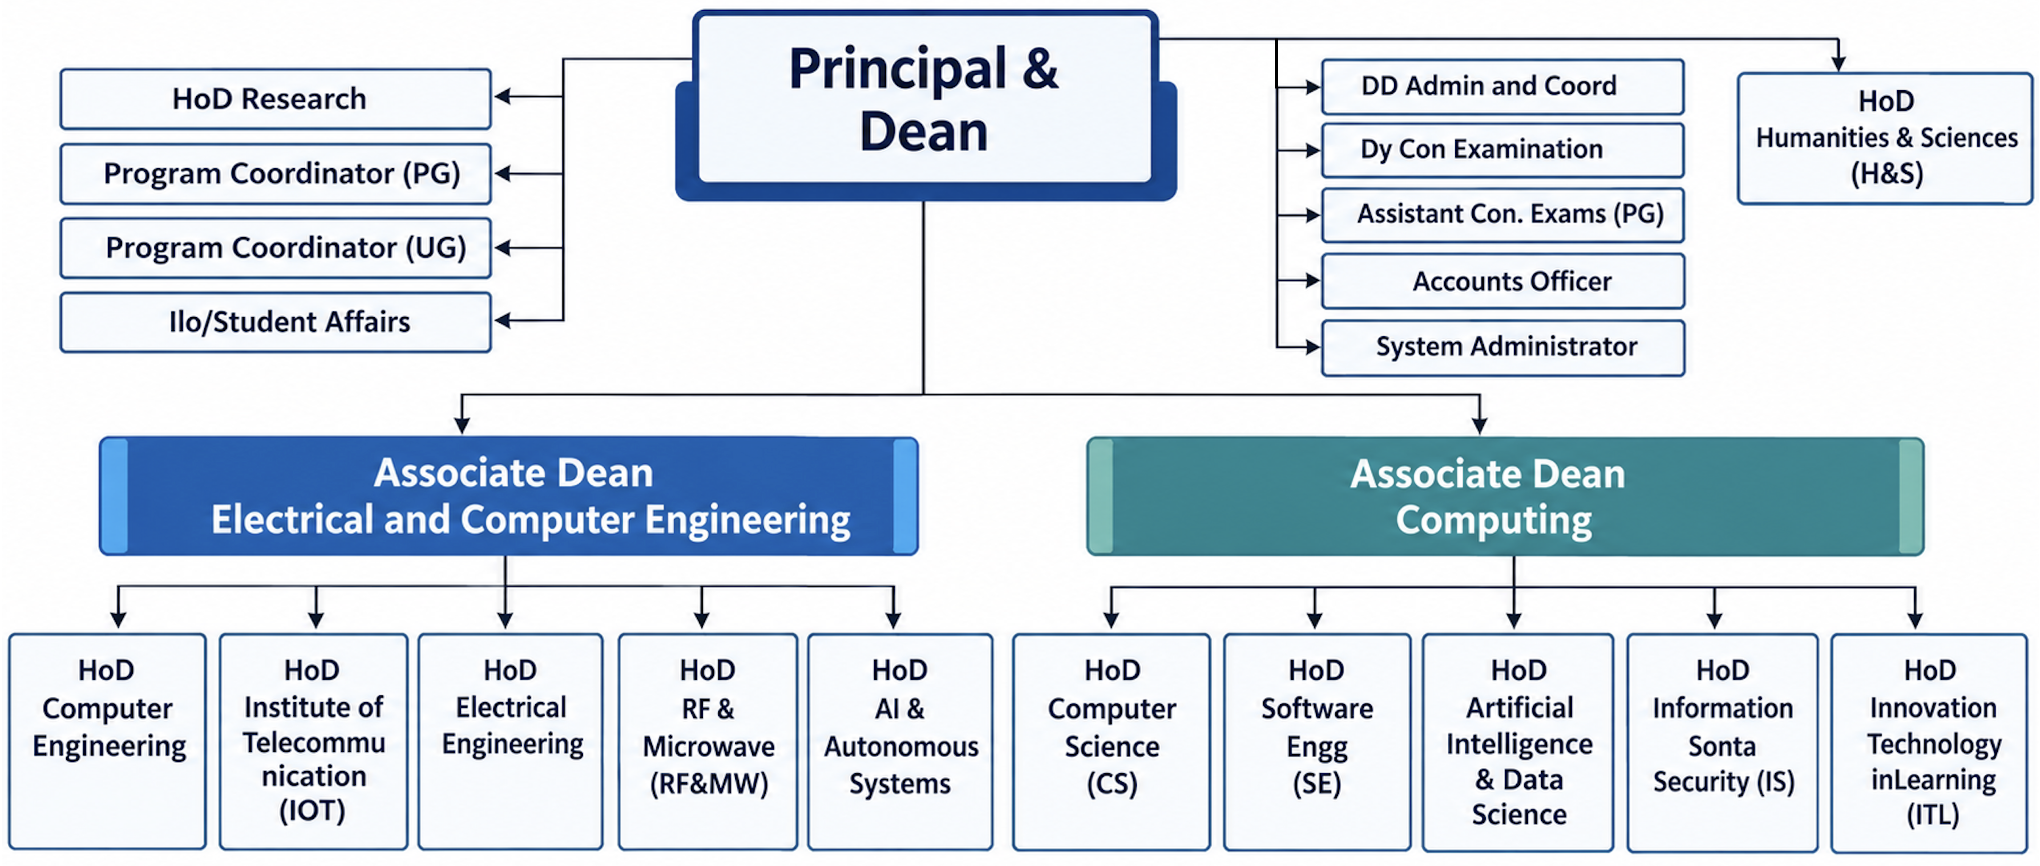
\includegraphics[width=1.0\textwidth]{images/front_matter/media/organogram.png}
    \caption{NUST-SEECS Organization}
    \label{fig:organ}
\end{figure}
\section{Accreditation History}\label{accreditation-history}

The BE Software Engineering program has undergone periodic accreditation and review by the Pakistan Engineering Council (PEC). Its accreditation history is summarized in Table~\ref{tab:history}.
\begingroup
\scriptsize
\setlength{\tabcolsep}{2pt}
\renewcommand{\arraystretch}{1.12}
\begin{longtable}{@{}>{\raggedright\arraybackslash}p{0.25\textwidth}>{\raggedright\arraybackslash}p{0.25\textwidth}>{\raggedright\arraybackslash}p{0.46\textwidth}@{}}
\caption{Accreditation History of BE Software Engineering Program}
\label{tab:history}\\
\toprule
\textbf{Date of Visit} & \textbf{Purpose} & \textbf{Remarks}\tabularnewline
\midrule
\endfirsthead
\toprule
\textbf{Date of Visit} & \textbf{Purpose} & \textbf{Remarks}\tabularnewline
\midrule
\endhead
\hline
September 2010 & Zero visit & Commencement of program approved\tabularnewline
\hline
24 June 2013 & Change of Scope & SEECS allowed to admit 2 sections\tabularnewline
\hline
18--19 June 2014 & Accreditation visit & Batch of 2010 accredited\tabularnewline
\hline
18--19 February 2016 & Accreditation visit & Batches of 2011 and 2012 
accredited\tabularnewline
\hline
22--24 February 2017 & Accreditation visit & Program accredited for two years (Batches 2013 and 2014)\tabularnewline
\hline
17--18 October 2018 & Accreditation visit & Program accredited for three years (Batches 2015, 2016, and 2017)\tabularnewline
\hline
14--15 March 2022 & Accreditation visit & Program accredited for two years (Batches 2018 and 2019)\tabularnewline
\hline
30--31 October 2023 & Accreditation visit & Program accredited for three years (Batches 2020, 2021, and 2022)\tabularnewline
\bottomrule
\end{longtable}
\endgroup

\section{Gap Analysis and Major Improvement Actions}\label{gap-analysis-for-implementation-of-obe-system}

The current review consolidates formal gaps recorded in the updated \emph{Gap Analysis} document and improvement needs addressed during the current accreditation cycle (Table~\ref{tab:gap-analysis-obe-current}). It distinguishes gaps identified through OBE review and previous PEC observations from subsequent program-level improvements documented in the 2026 SAR, reflecting progress beyond the initial 2014 OBE transition through PEC observations, internal CQI, Industrial Advisory Board (IAB) feedback, curriculum working papers, and institutional investment. These subsequent initiatives are presented as improvement needs, not new PEC deficiencies. Responses to previous PEC observations are consolidated in the \textbf{Rejoinder} under Criterion 8, while implementation evidence is provided under the relevant criteria and annexures to avoid duplication in Chapter 1.

\begingroup
\footnotesize
\setlength{\tabcolsep}{4pt}
\renewcommand{\arraystretch}{1.14}
\begin{longtable}{@{}>{\centering\arraybackslash}p{0.05\textwidth}>{\raggedright\arraybackslash}p{0.38\textwidth}>{\raggedright\arraybackslash}p{0.51\textwidth}@{}}
\caption{Expanded Gap Analysis and Major Improvement Actions}
\label{tab:gap-analysis-obe-current}\\
\toprule
\textbf{S. No.} & \textbf{Gap / Improvement Need} & \textbf{Action Taken / Current Status}\\
\midrule
\endfirsthead
\toprule
\textbf{S. No.} & \textbf{Gap / Improvement Need} & \textbf{Action Taken / Current Status}\\
\midrule
\endhead
\midrule
\multicolumn{3}{r}{\footnotesize\itshape Continued on next page}\\
\endfoot
\bottomrule
\endlastfoot

1 & The Alumni and Employer Survey
instruments required stronger and
more balanced alignment with the
Program Educational Objectives (PEOs) Key Performance Indicators
(KPIs). & The Alumni and Employer Surveys were redesigned in 2026 to strengthen alignment with PEO KPIs, each comprising 12 five-point Likert items, with four dedicated to each PEO. The instruments were approved by Department Board of Studies (DBS) on 20 April 2026 and Faculty Board of Studies (FBS) on 21 April 2026, and endorsed by IAB on 5 May 2026. Pilot normalized PEO scores were 0.803, 0.797, and 0.803, confirming attainment of all three PEOs. This addresses a previous PEC concern discussed in (Criteria 1 and 8 \& Rejoinder).\\
\addlinespace[2pt]
2 & The legacy PEO evaluation framework and follow-up mechanism required clearer, more traceable corrective-action logic. & A transparent multi-step PEO evaluation framework was introduced, covering question-level KPI checks, indicator coverage, and normalized PEO scoring. Corrective actions are tracked through a standard Corrective Action Form, ensuring an auditable CQI trail.\\
\addlinespace[2pt]
3 & The Graduate Exit Survey provided limited direct traceability between survey questions and individual Program Learning Outcomes (PLOs). & The Graduate Exit Survey was redesigned with each item mapped to a specific PLO and deployed through the Learning Management System (LMS), providing structured, PLO-wise indirect evidence for recent graduating batches (Criteria 2 and 8).\\
\addlinespace[2pt]
4 & Internship feedback provided insufficiently structured indirect PLO evidence and depended on a largely manual collection process. & The Internship Employer Feedback Form was redesigned with direct PLO mapping and integrated into the Online Internship Module. Combining employer feedback with faculty assessment provides traceable dual-source evaluation and addresses the previous PEC observation on indirect assessment (Criteria 2, 3, 8, and Rejoinder).\\
\addlinespace[2pt]
5 & The Software Engineering PLO framework required alignment with the revised PEC/HEC graduate attributes, which reduced the number of graduate attributes from 12 to 11. & The BESE PLO framework was revised from 12 to 11 to align with current PEC requirements, consolidating society and sustainability attributes within the revised graduate-attribute structure and updating the remaining PLOs. Batch-specific implementation and mapping are documented in Criterion 2 and the approved curriculum working papers.\\
\addlinespace[2pt]
6 & The curriculum required periodic regulatory alignment with successive PEC/HEC Undergraduate Education Policy updates and NUST academic requirements. & Three major curriculum working papers were processed: the 64th ACM (2023) redistributed FYDP credit hours; the 69th ACM (2024) incorporated UEP-2023 requirements, including the revised PLO structure and updated non-engineering courses requirements. Details are provided in Criterion 3; and the 72nd ACM (2025) incorporated UEP-2024 changes\\
\addlinespace[2pt]
7 & The program required broader field-specific elective choice and strengthening of the programming foundation. & Engineering electives were increased from five to six, with emerging offerings including Virtual and Augmented Reality, Introduction to Quantum Computing, Large Language Models, and Reinforcement Learning. Fundamentals of Computer Programming course credit hours were increased from 3 to 4 and Applications of ICT was introduced to strengthen computing/programming foundations of fresh intake. These changes reflect curriculum review and IAB recommendations (Criteria 3 and 9).\\
\addlinespace[2pt]
%8 & A formal academic mechanism for recognizing validated professional/certification-based learning was not available. & NUST Working Paper No. 2 of the 73rd ACM approved a framework for departmentally validated certification-style courses carrying 1--3 credit hours. The initiative has institutional approval but remains subject to the final PEC Engineering Accreditation Board SOP. \textbf{Status: Partially implemented / awaiting PEC SOP.}\\
%\addlinespace[2pt]
8 & Complex Engineering Problems (CEP) required a documented and consistently applied departmental mechanism across relevant courses. & A formal departmental CEP policy was documented and disseminated, requiring courses with laboratories/projects to incorporate relevant CEP elements addressing complex problem formulation, analysis, and solution development. Policy and implementation evidence are provided in Criterion 3.\\
\addlinespace[2pt]
9 & Open-Ended Laboratory (OEL) practice required more systematic institutionalization. & OEL activities were institutionalized in relevant laboratory courses, requiring students to develop methodologies, justify engineering decisions, and validate solutions beyond predefined procedures. Supporting policies and examples are provided in Criterion 3.\\
\addlinespace[2pt]
10 & Internship mechanism needed to be strengthened as a structured component of professional preparation and graduation requirements. & A 6–8-week internship is now mandatory for BESE graduation, supported by SEECS Industry Liaison Office (ILO) and NUST Placement Office (NPO) placement coordination. The LMS module enables digital feedback collection, complemented by employer and faculty evaluations (Criteria 3, 4, and 8).\\
\addlinespace[2pt]
11 & Faculty required continuing development in OBE implementation, particularly CLO formulation, Bloom's Taxonomy, PLO mapping, CEP and OEL. & 
Department-level OBE training is conducted at the start of each semester for all faculty, including new, continuing, and TVF members. Newly inducted faculty also receive mandatory one-week HR-led onboarding, with OBE training as a core module. Additional post-PEC sessions were conducted to strengthen faculty's taxonomy-level understanding. Institutional funding supports pedagogical training, certifications, and conference participation (Criteria 5, 7, and 8).\\
\addlinespace[2pt]
12 & Course outlines required comprehensive CLO--PLO mapping and explicit identification of appropriate teaching and assessment methods. & Course outlines and CLO–PLO mappings are periodically revised through faculty knowledge heads and CQI reviews. Each Course Learning Outcome (CLO) is linked to appropriate direct and/or rubric-based assessments, with course and laboratory folders maintained on the LMS for traceability and review.\\
\addlinespace[2pt]
13 & Some CLOs/courses were mapped at lower or inappropriate Bloom's Taxonomy levels, requiring stronger taxonomy alignment. & CLO wording and taxonomy levels are periodically reviewed and revised through course-level and departmental CQI processes.\\
\addlinespace[2pt]
14 & CQI actions required a more consistent institutional mechanism for ownership, documentation, follow-up and closure. & A dedicated CQI Committee reviews assessment results and monitors corrective actions. A standardized Corrective Action Form tracks actions, responsibilities, follow-up, and closure across curriculum, CLO, PLO, and PEO improvements, ensuring an auditable record (Criterion 8 and relevant annexures).\\
\addlinespace[2pt]
15 & OBE records and attainment analysis required sustainable digital documentation and reliable semester-/batch-wise reporting. & Course and laboratory folders are maintained on the LMS, while NUST’s Qalam OBE system generates semester- and batch-wise CLO/PLO attainment reports, strengthening record continuity, auditability, and data-driven CQI (Criteria 2, 3, and 8).\\
\addlinespace[2pt]
%17 & Students with weak individual PLO attainment required an explicit monitoring and recovery mechanism before graduation. & Individual PLO performance is monitored through Qalam. Students with identified deficiencies receive advisory or warning communication depending on stage of study, and additional/recovery learning is arranged where required. Full PLO attainment is checked as part of degree-completion monitoring. See Criteria 2 and 4.\\
%\addlinespace[2pt]
16 & SEECS had active industry collaboration, but a formal mechanism for recording and monitoring industry-sponsored FYDPs was missing. & TMS now records industry-sponsored FYDPs and co-supervision by SEECS faculty and industry/NSTP professionals, providing a formal digital audit trail. The platform also maintains internship evidence (Criteria 8 and 9).\\
%\addlinespace[2pt]
%19 & Industry input needed to translate more systematically into documented program and curriculum improvements. & The Industrial Advisory Board has met regularly during the accreditation cycle. The initiatives review records eight IAB sessions from May 2023 to May 2026, with 20 recommendations and 12 closed actions. Closed items include new electives, strengthening of programming credit hours and revision of PEO assessment instruments. See Criteria 1 and 9.\\
\addlinespace[2pt]
17 & Physical and computing infrastructure required expansion and modernization to support growing academic, laboratory and project needs. & The new SEECS Academic Block adds 14 classrooms, six teaching laboratories, three FYDP laboratories, faculty and officer offices, and supporting academic spaces. Computing facilities were further strengthened through the procurement of 45 new PCs and upgrades to 50 existing PCs.\\
\addlinespace[2pt]
18 & Network access and supporting digital/library infrastructure required continued strengthening for teaching, research and remote access. & SEECS has 910 Mbps PERN connectivity through the NUST campus core network, a 7 Mbps backup for research laboratories, and VPN-based remote access. Library facilities include high-speed internet, Wi-Fi, group study rooms, and academic spaces (Criteria 6 and 7).\\
\addlinespace[2pt]
19 & Student support made more integrated, accessible mechanisms covering administrative facilitation, counselling and employability. & NUST has introduced/strengthened centralized support through the Student Support Services Centre (S3C), the Centre for Counselling and Career Advisory (C3A), and the Career Development Centre (CDC). These provide one-window facilitation, professional counselling/career assessment, employability development and employer engagement. See Criteria 4, 6 and 9.\\
\end{longtable}
\endgroup

%\section{Historical Review of OBE Implementation}\label{historical-review-of-obe-implementation}

%SEECS initiated its formal transition to Outcome-Based Education (OBE) in June 2014 in response to the PEC Manual of Accreditation 2014. The first phase focused on defining and approving the program Mission, PEOs and PLOs, followed by faculty awareness and training on OBE principles, CLO--PLO mapping, Bloom's Taxonomy, course-outline design, teaching methods and assessment practices. These activities led to the adoption of OBE-aligned course outlines and assessment practices from Fall 2014 onward.

%The implementation was subsequently strengthened through continued faculty development, periodic accreditation reviews and the introduction of supporting academic systems. QOBE software was introduced in 2016 to facilitate management of outcome-based assessment data. Engagement with the Industrial Advisory Board and formal CQI meetings further supported review of curriculum relevance and attainment results. Workshops on emerging OBE practices continued, and newly inducted faculty were provided OBE orientation to maintain consistency in implementation.

%By 2021, OBE processes had become integrated with the institutional academic management framework through training on QALAM and routine use of the program's Quality Management System. The historical progression from initial OBE adoption to a structured CQI-based system established the foundation for the present assessment, review and corrective-action mechanisms described in the subsequent criteria of this SAR.

\section{Quality Management System}\label{quality-management-system}

The NUST Quality Management System (QMS) comprises various entities responsible for monitoring, managing, and enhancing academic quality in accordance with NUST statutes, policies, and associated addenda. The Software Engineering Department at SEECS has implemented an OBE-focused QMS (Figure~\ref{fig:qms}), operating through a hierarchical structure comprising the Local Quality Enhancement Cell (LQEC), Department Board of Studies (DBS), Faculty Board of Studies (FBS), University Curriculum Review Committee (UCRC), and Academic Council Meeting (ACM).
\begin{figure}[!hb]
\centering
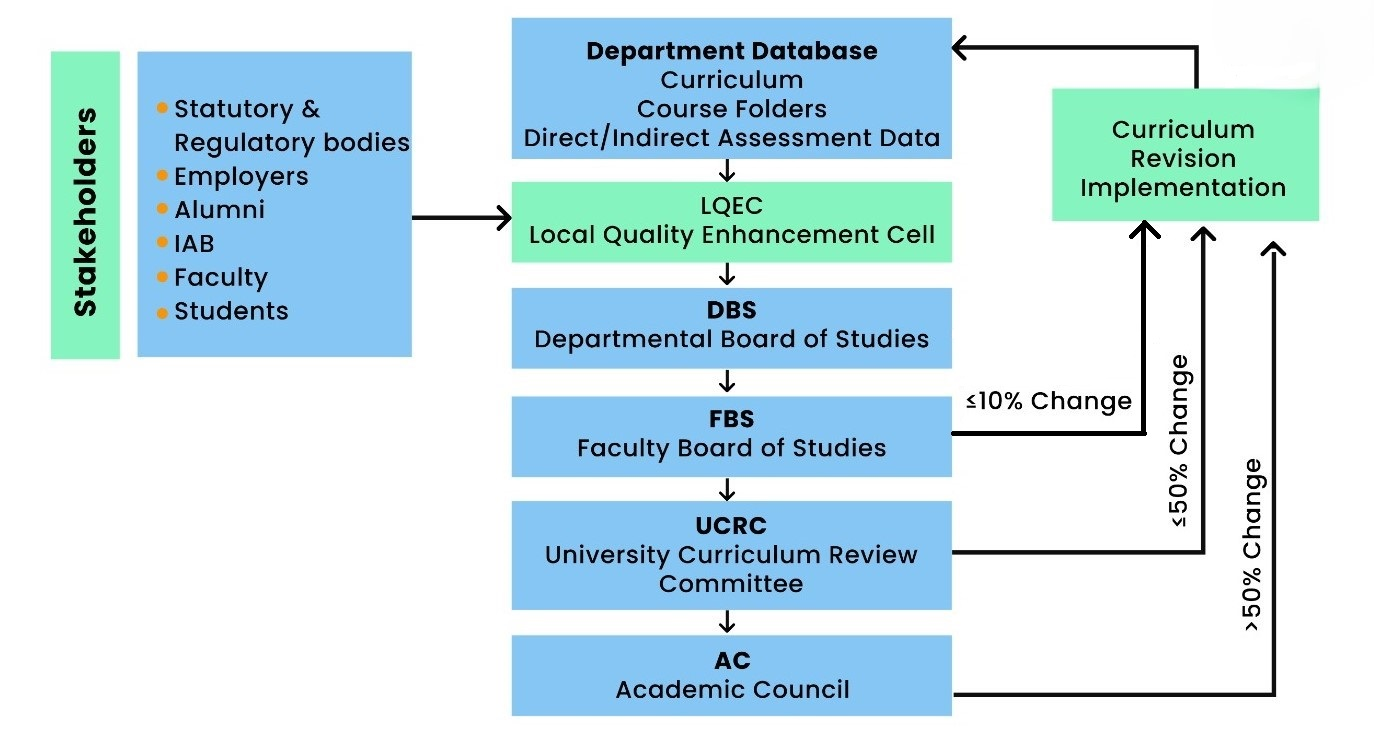
\includegraphics[width=1.0\textwidth]{images/criterion_8/media/Curr_review.jpeg}
\caption{Quality Management System (QMS)}
\label{fig:qms}
\end{figure}

\subsection{Local Quality Enhancement Cell (LQEC)}\label{local-quality-enhancement-cell}

Local Quality Enhancement Cell (LQEC) is composed of a nominated faculty member responsible for quality assurance of the program. It oversees the quality assessment process being carried out for the program. The LQEC is assisted by Knowledge Group Heads who make sure the course outline and exams are according to the guidelines. The primary role of LQEC is to analyze data collected from various sources such as exams/rubrics, various surveys and feedback. LQEC invokes corrective action process in case of deficiency observed because of CQI. Figure~\ref{fig:pqms} shows the flowchart for a typical CQI process for all levels of the program.

\begin{figure}[!hb]
\centering
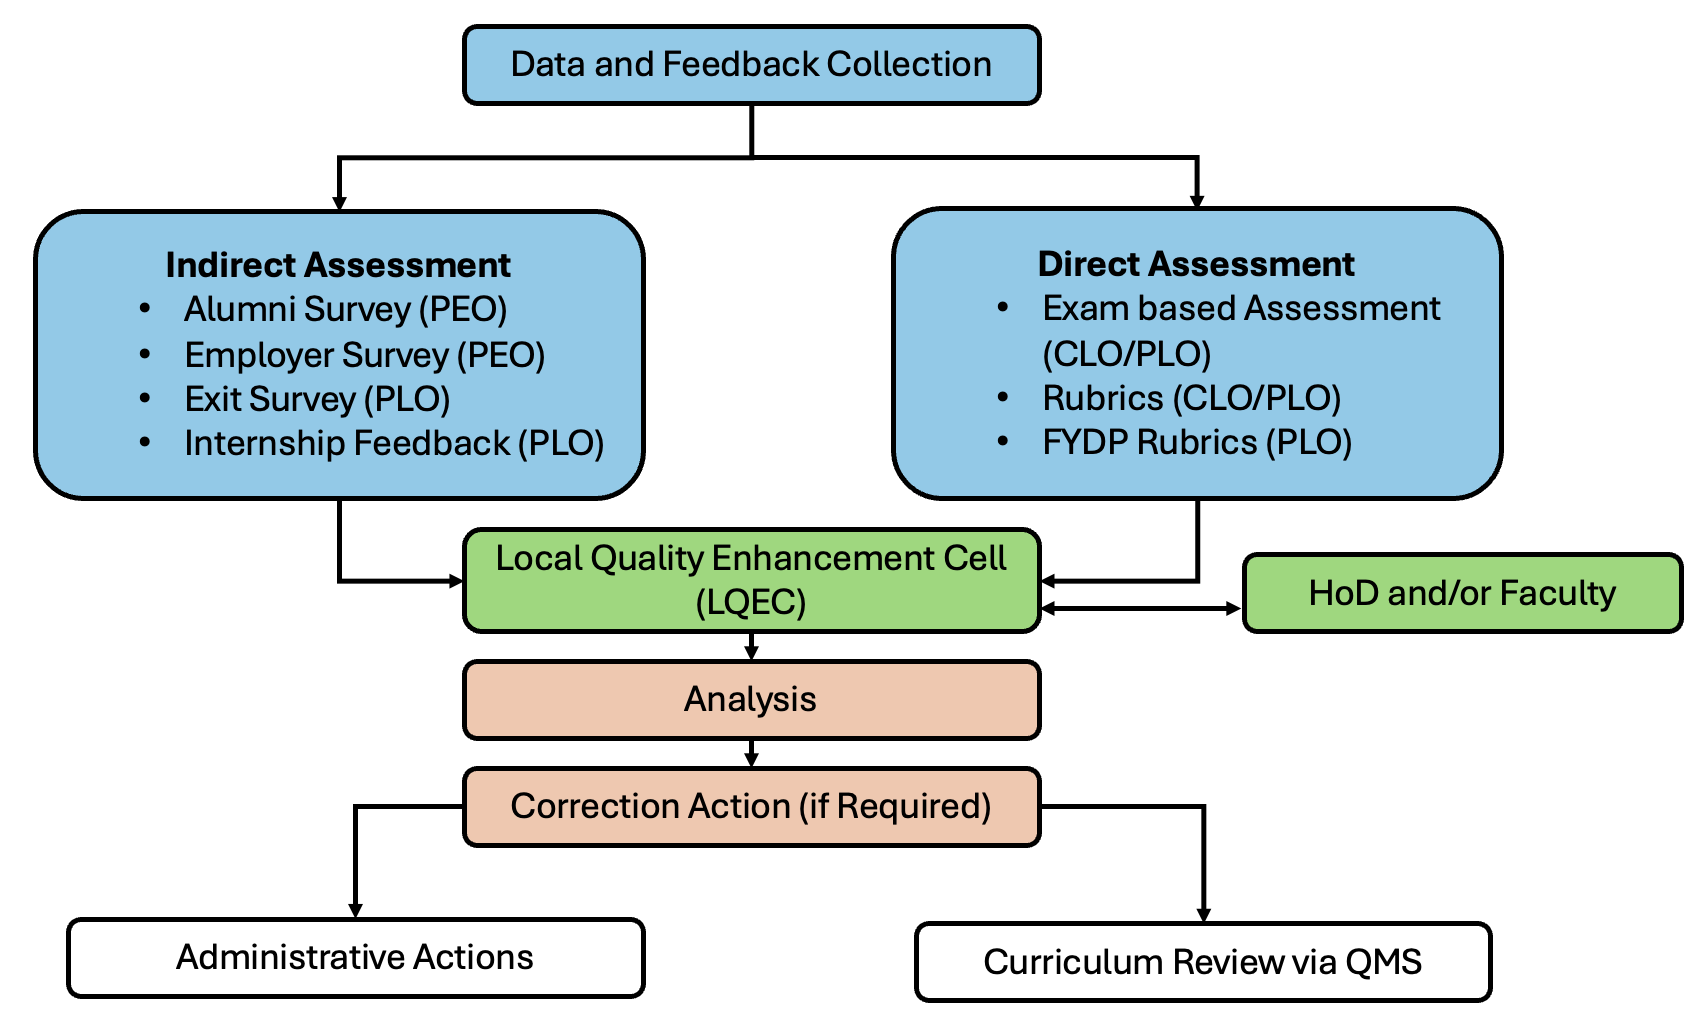
\includegraphics[width=1.0\textwidth]{images/front_matter/media/image-5.png}
\caption{Program Quality Assurance Process}
\label{fig:pqms}
\end{figure}

\subsection{Department Board of Studies}\label{department-board-of-studies}

Department Board of Studies (DBS) is composed of Associate Dean (Chairman), LQEC, all Heads of Departments (HoDs), program coordinator and assistant controller exams. The meeting is convened to present results, attainment of CLOs, PLOs and PEOs for different batches and to initiate any changes if required.

\subsection{Faculty Board of Studies}\label{faculty-board-of-studies}

Faculty Board of Studies (FBS) is composed of Principal SEECS, both Associate Deans of SEECS, all HoDs of SEECS, Deputy Controller Exams, and representatives from NUST main office. Any changes resulting from corrective actions in curricula up to 10\% are approved in FBS and implemented. More than 10\% of changes are approved for presentation in UCRC.

\subsection{University Curriculum Review Committee}\label{university-curriculum-review-committee}

University Curriculum Review Committee (UCRC) is composed of Pro Rector Academics (Chairman), Registrar, Director QA, Director PGP, Principal SEECS, Associate Dean Computing, Industrial Representatives, Director Research and Director Academics. Changes in curriculum up to 50\% are approved in UCRC. More than 50\% are approved for presentation in Academic Council Meeting.

\subsection{Academic Council}\label{academic-council}

Academic Council (AC) is composed of Rector NUST (Chairman), Pro Rector Academics, Pro Rector P\&R, Registrar, Principals or Deans of all Schools, Director QA, Directors of all NUST Directorates, and Industrial Representatives, as needed. Any major changes (more than 50\%) forwarded by UCRC are discussed and approved by Academic Council.

\section{Industry Advisory Board (IAB)}\label{industry-advisory-board-iab}

In addition to the several bodies discussed above, SEECS holds regular meetings of the board of industry representatives and alumni. This board provides a formal platform for interaction with industrial experts and alumni to provide feedback about the program, its direction, curriculum, and any other related matters.

\section{Corporate Advisory Council (CAC)}\label{corporate-advisory-council-cac}

The CAC was formed in 2010 under chairmanship of Rector to create a positive impact on the socio-economic development of Pakistan through active engagement with the industry. The CAC has been instrumental in developing linkages with industrial and business enterprises across multiple sectors of the economy.

%\paragraph{Facilities and safety evidence.} Detailed information on institutional facilities, workplace safety, fire-safety arrangements, and supporting evidence is presented under Criterion 6 and is not duplicated in the Introduction.

\section{OBE Implementation Model}\label{obe-implementation-model}

The OBE implementation model is a continuous process in which the attainment of the Program Mission and PEOs is monitored through indirect assessments. SEECS formally initiated OBE implementation in June 2014 in response to the PEC Manual of Accreditation 2014, followed by faculty training and the adoption of OBE-aligned course outlines and assessment practices. Implementation was strengthened through continued faculty development, the introduction of QOBE software in 2016, engagement with the Industrial Advisory Board (IAB), and formal Continuous Quality Improvement (CQI) reviews. By 2021, OBE processes had been integrated into academic management through QALAM training and the routine use of the program's Quality Management System. The flowchart in Figure~\ref{review of PEOs} illustrates the CQI process through three interconnected loops: the outermost loop monitors PEO attainment and overall program success, the middle loop assesses PLO attainment, and the innermost loop evaluates CLO attainment. Each loop follows four steps i.e. data collection, evaluation, review, and corrective action.
\begin{figure}[H]
\centering
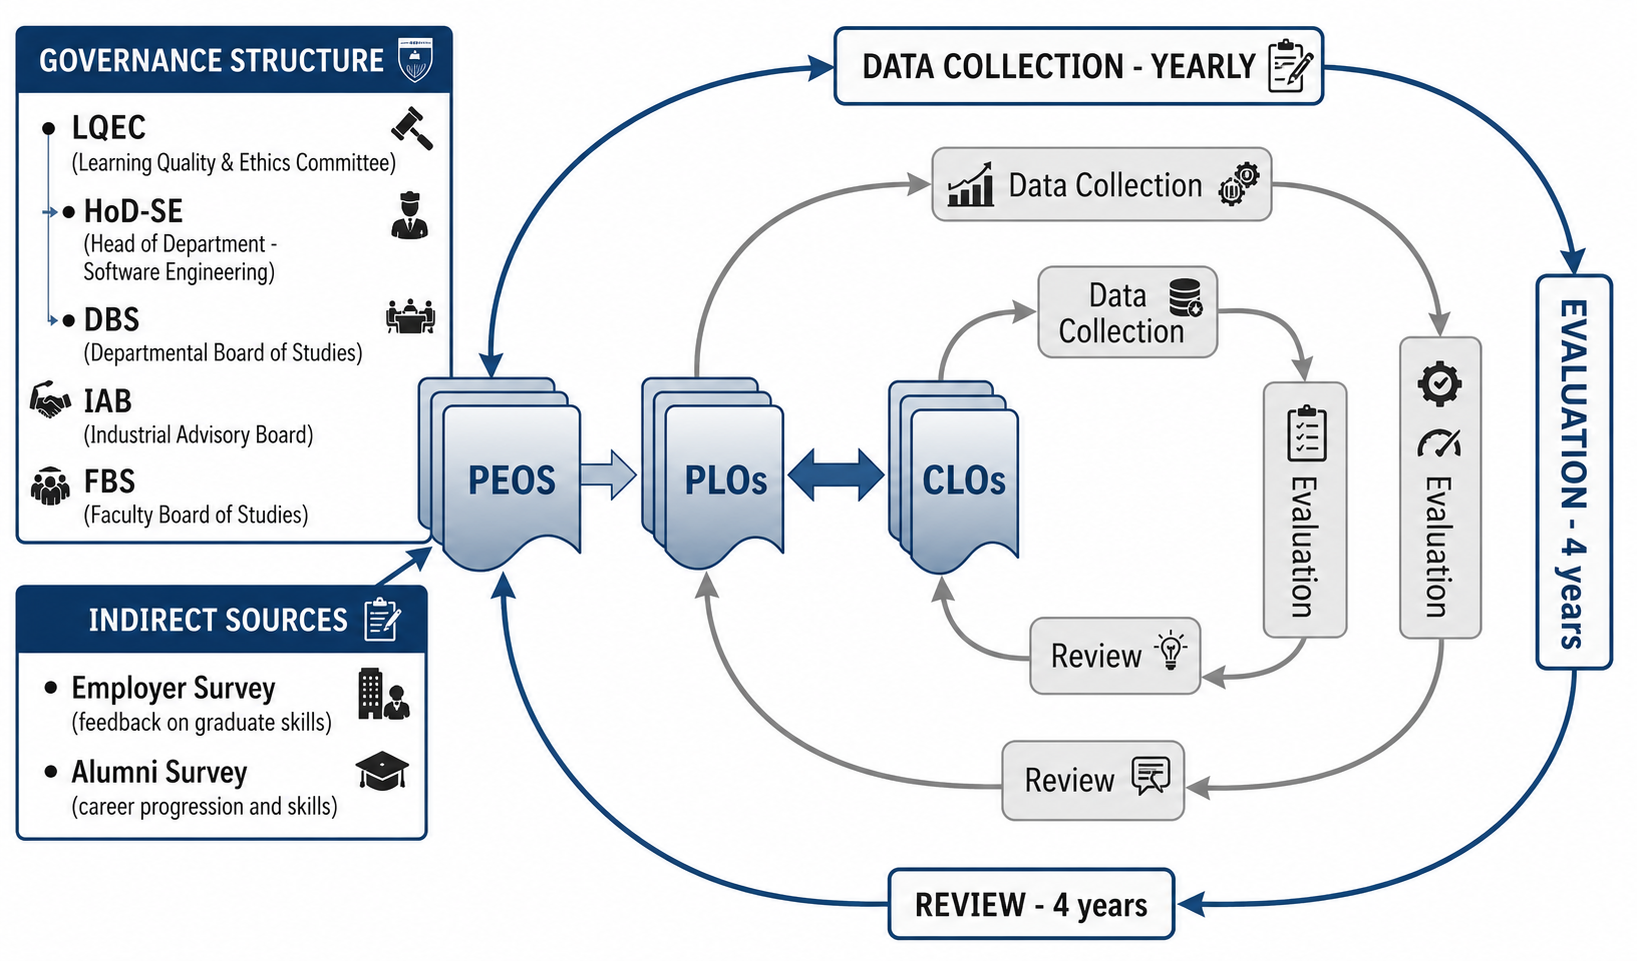
\includegraphics[width=1.0\textwidth]{images/front_matter/media/image13.png}
\caption{CQI Process through Three Interconnected Loops}
\label{review of PEOs}
\end{figure}
\subsection{CQI Process for PEOs}\label{peos}
%\subsubsection{CQI Process for PEOs}\label{cqi-process-for-peos}

The LQEC is responsible for the initiation of CQI for attainment, revision, and improvement of PEOs. PEOs are indirectly assessed through alumni and employer surveys, with data collected yearly and review carried out four years after graduation of each batch. The review process starts with measurement of PEOs and involves CQI, corrective actions and administrative processes for maintenance and/or improvement of PEOs as shown in Figure~\ref{fig:corrective action processes for PEOs}. If the achievement of PEOs is attained, no corrective action is required; otherwise, the CQI process is invoked by LQEC.

\begin{figure}[H]
\centering
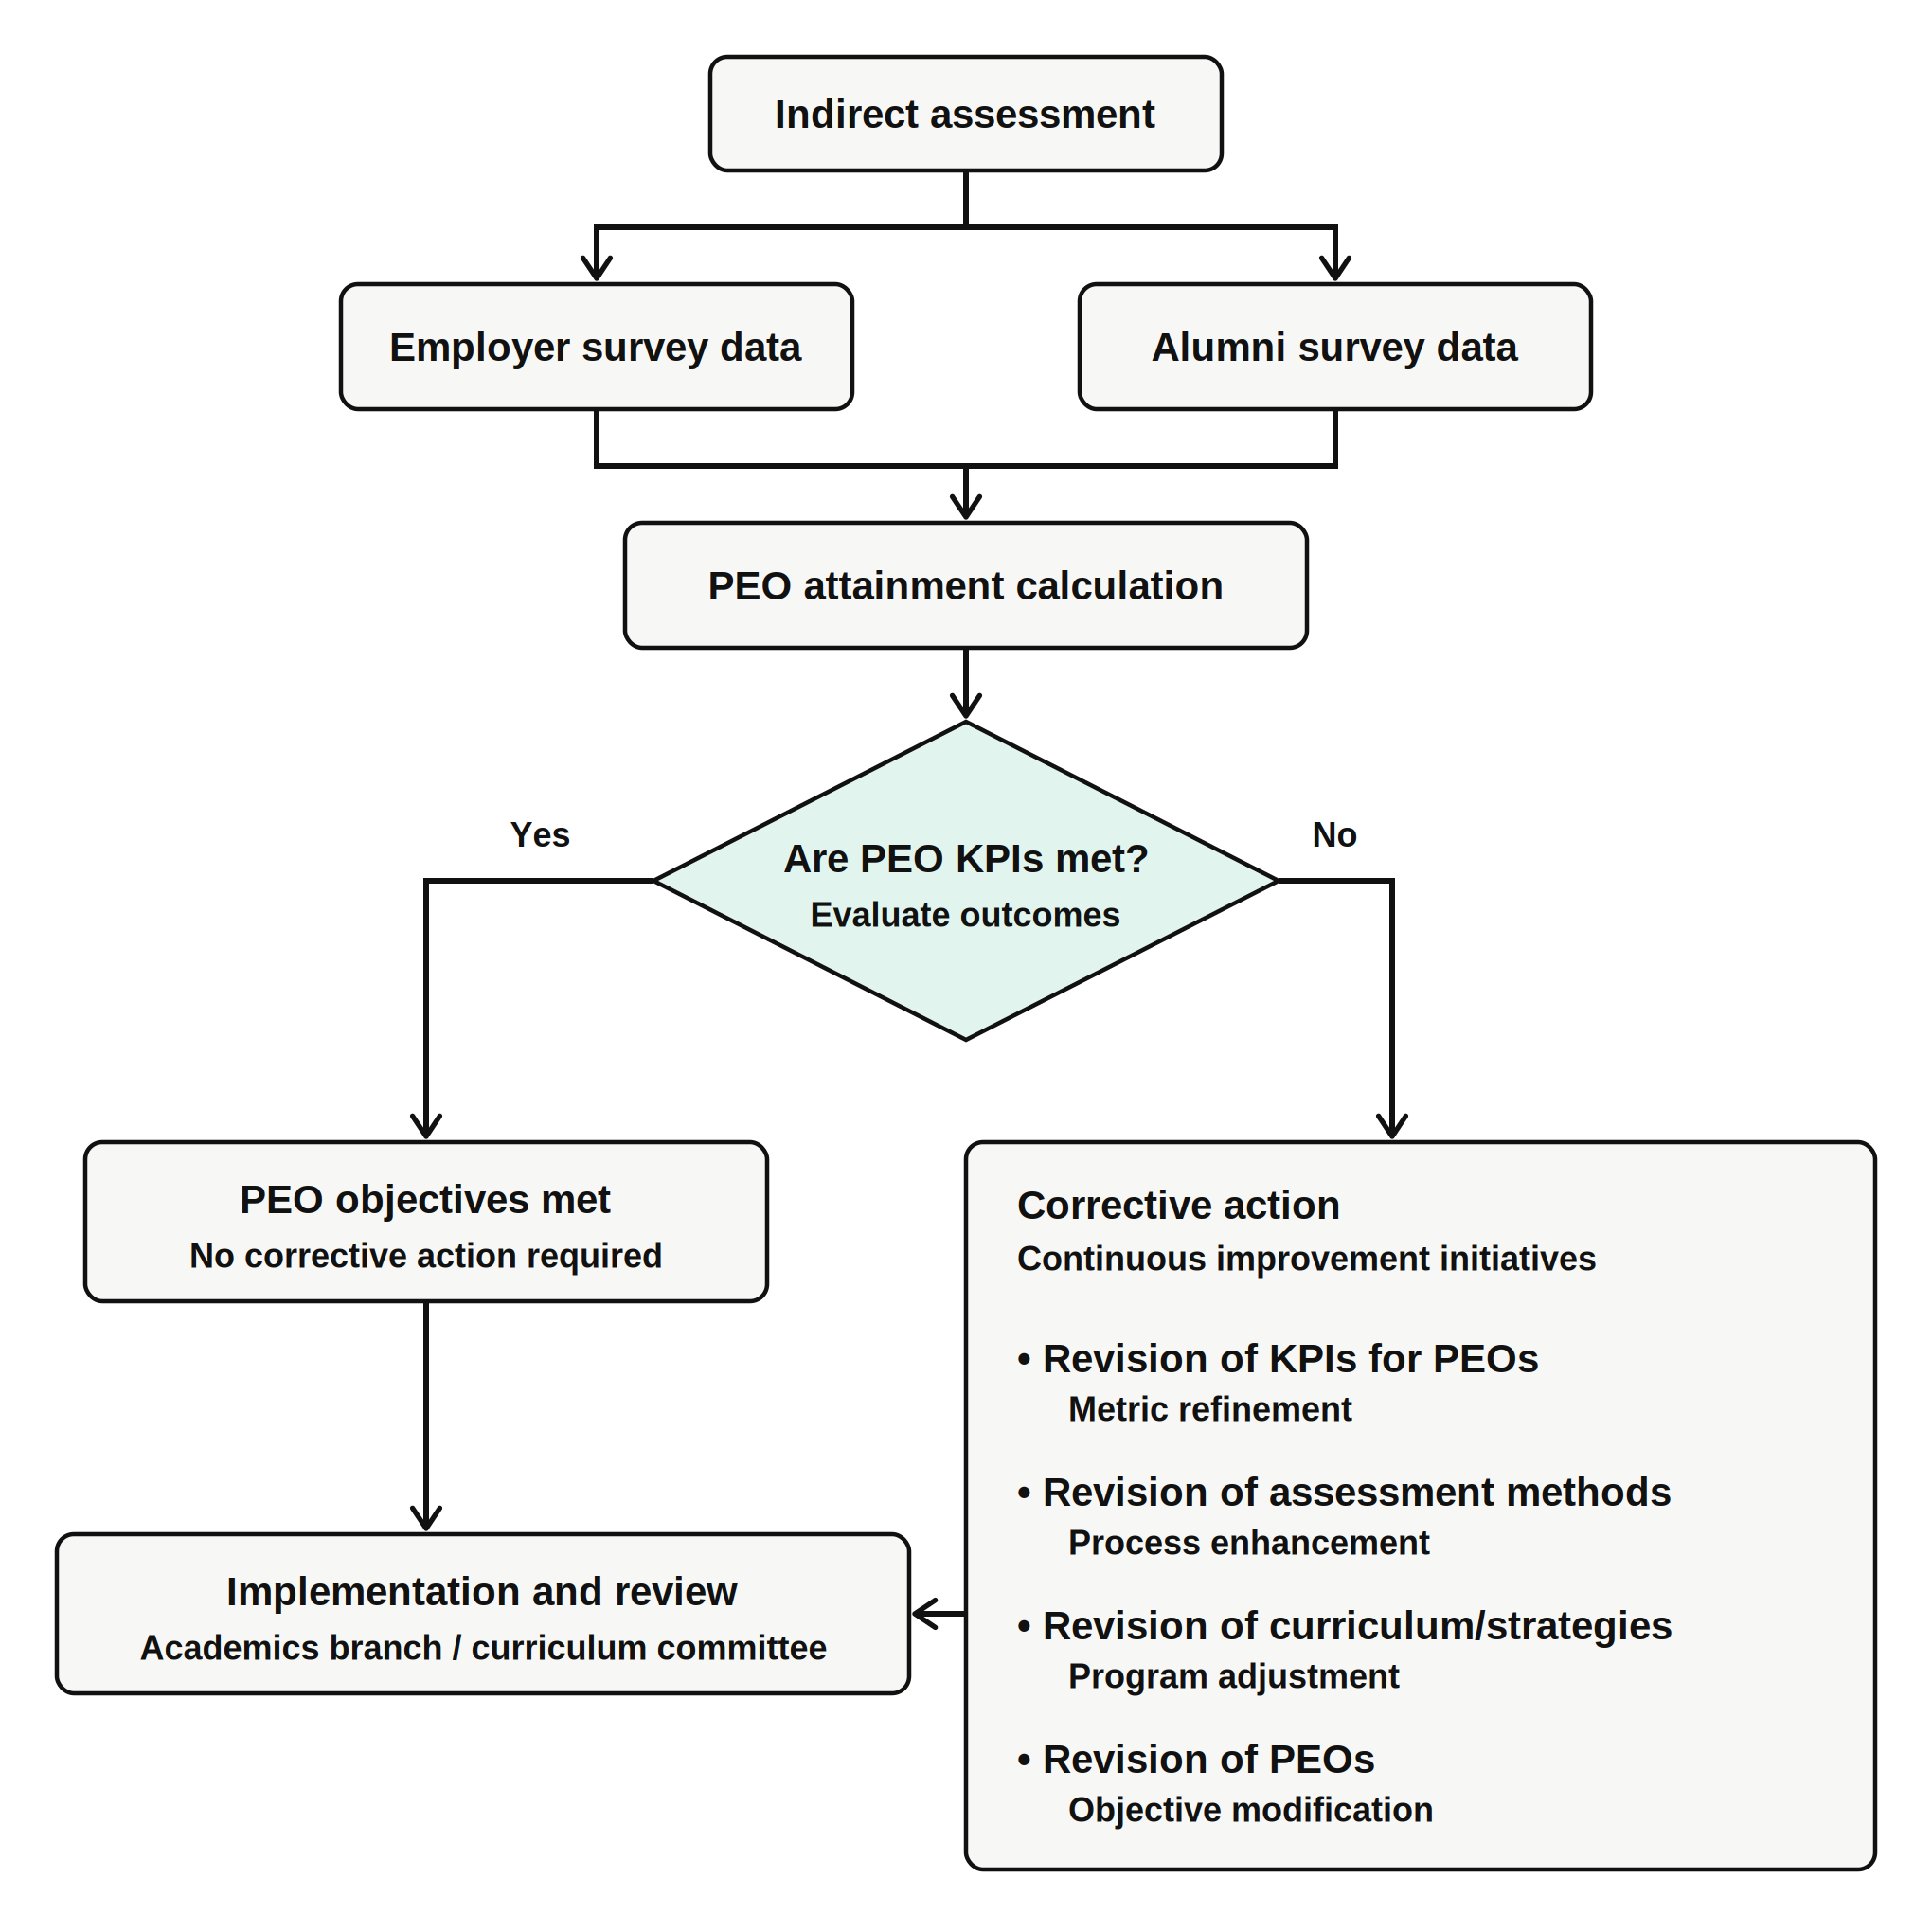
\includegraphics[width=0.89\textwidth]{images/front_matter/media/image-14.png}
\caption{Flowchart Showing Review \& Corrective Action Processes for PEOs}
\label{fig:corrective action processes for PEOs}
\end{figure}
%\subsubsection{Review and Corrective Action Processes for PEOs}\label{review-and-corrective-action-processes-for-peos}

\subsection{CQI Process for PLOs}\label{plos}

%\subsubsection{CQI Process for PLOs}\label{cqi-process-for-plos}

LQEC is responsible for CQI process for evaluation and attainment of PLOs. PLOs are directly assessed through CLOs and Final Year Design Projects (FYDPs), whereas indirect assessment is done through internship feedback and exit surveys (Figure~\ref{fig:corrective action processes for plos}).  Figure~\ref{fig:individual-level1} and Figure~\ref{fig:cohort level}, show the review process for PLOs at individual and cohort levels respectively. Individual PLO analysis starts with direct assessment, where each student’s PLO attainment is calculated in their courses and then analysed against the respective KPI. If the KPI is met, no corrective action is needed. If the KPI is not met, the student moves through escalating stages. A counselling stage with a letter of advice comes after semesters 4–6. A warning stage with a warning letter comes after semester 7. If attainment is still short after semester 8, the special module stage applies, with another warning letter and the department arranging extra module(s) to help the student reach the PLO. 

\begin{figure}[H]
\centering
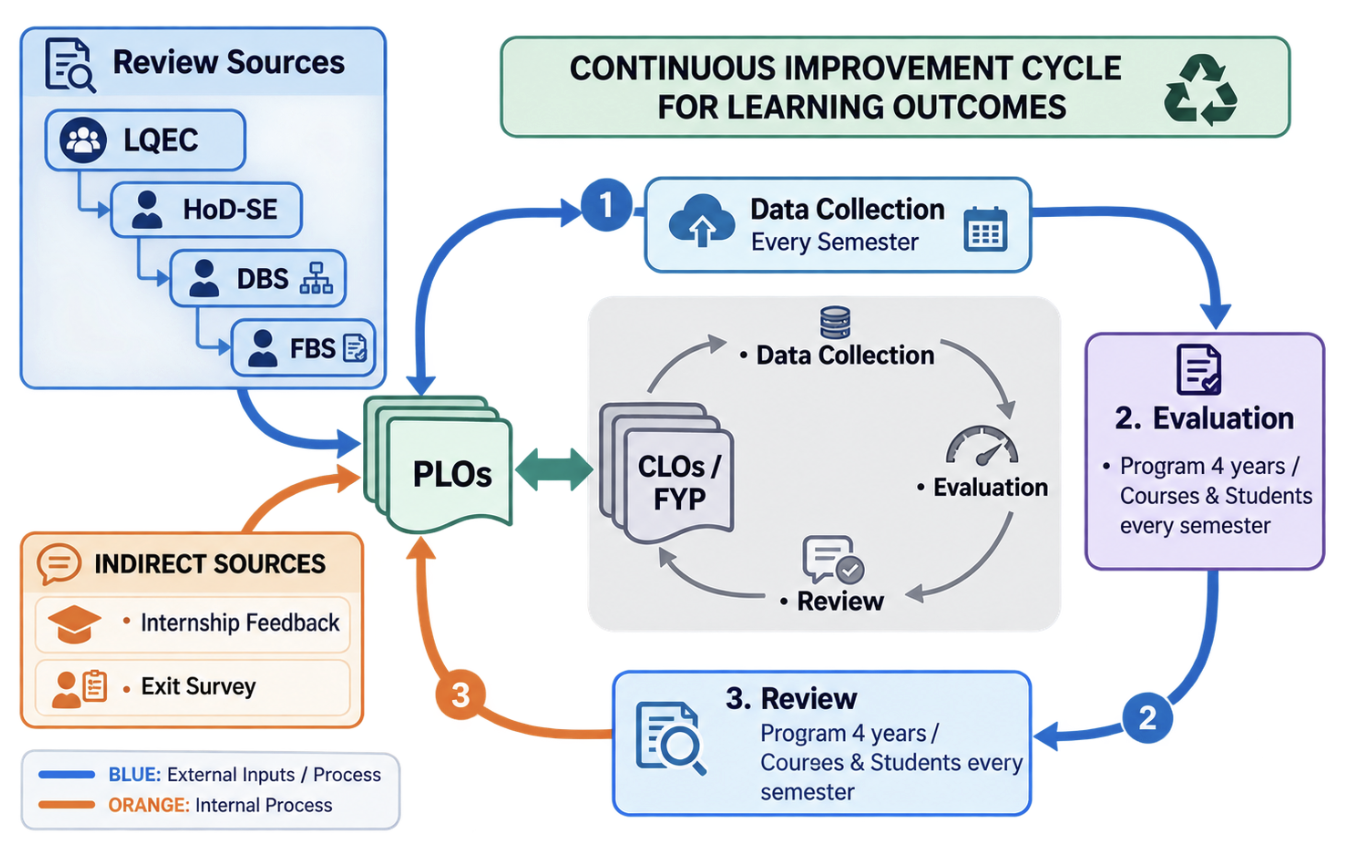
\includegraphics[width=0.88\textwidth]{images/front_matter/media/image-15.png}
\caption{Flowchart Showing Review \& Corrective Action Processes for PLOs}
\label{fig:corrective action processes for plos}
\end{figure}

For a cohort, if PLO attainment is more than or equal to 60\% as per KPI, no corrective action is required. Otherwise the CQI process invokes corrective actions including the revision of KPIs, CLO-PLO remapping, curriculum revision, and review of teaching \& learning processes.

%\subsubsection{Review and Corrective Action Processes for PLOs}\label{review-and-corrective-action-processes-for-plos}

\begin{figure}[H]
\centering
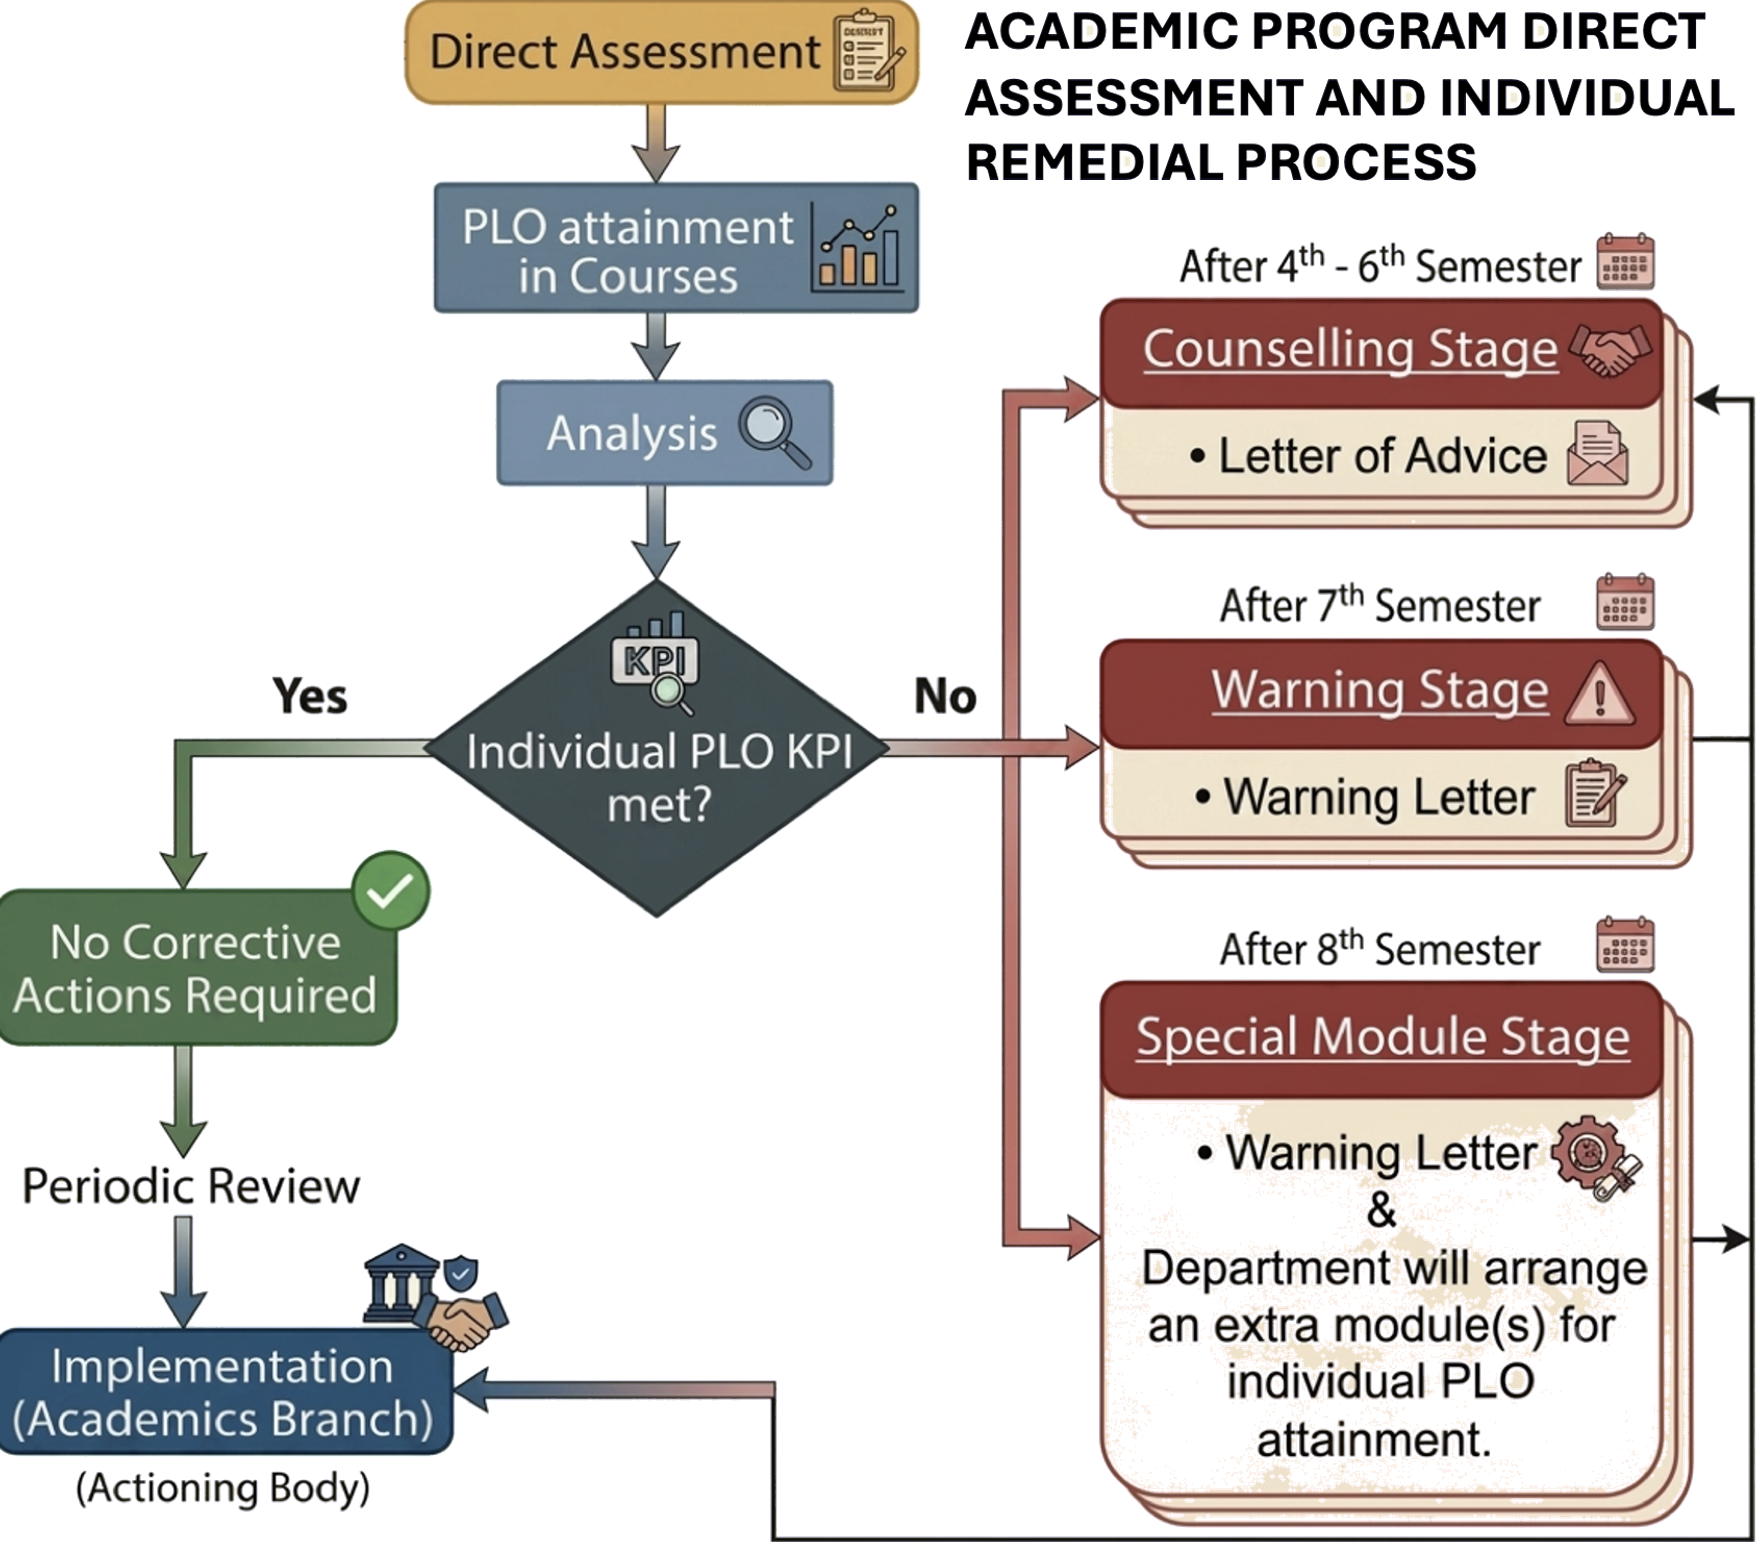
\includegraphics[width=0.7\textwidth]{images/front_matter/media/image-16.png}
\caption{Review of PLOs at Individual Level \& Corrective Actions}
\label{fig:individual-level1}
\end{figure}

\begin{figure}[H]
\centering
\includegraphics[width=0.8\textwidth]{images/front_matter/media/image17.png}
\caption{Review of PLOs at Cohort Level \& Corrective Actions}
\label{fig:cohort level}
\end{figure}

\subsection{CQI Process for CLOs}\label{clos}

%\subsubsection{CQI Process for CLOs}\label{cqi-process-for-clos}
The innermost loop of OBE implementation model deals with CQI process for CLOs (coursework) as shown in Figure~\ref{fig:cqi clo}. 
\begin{figure}[H]
\centering
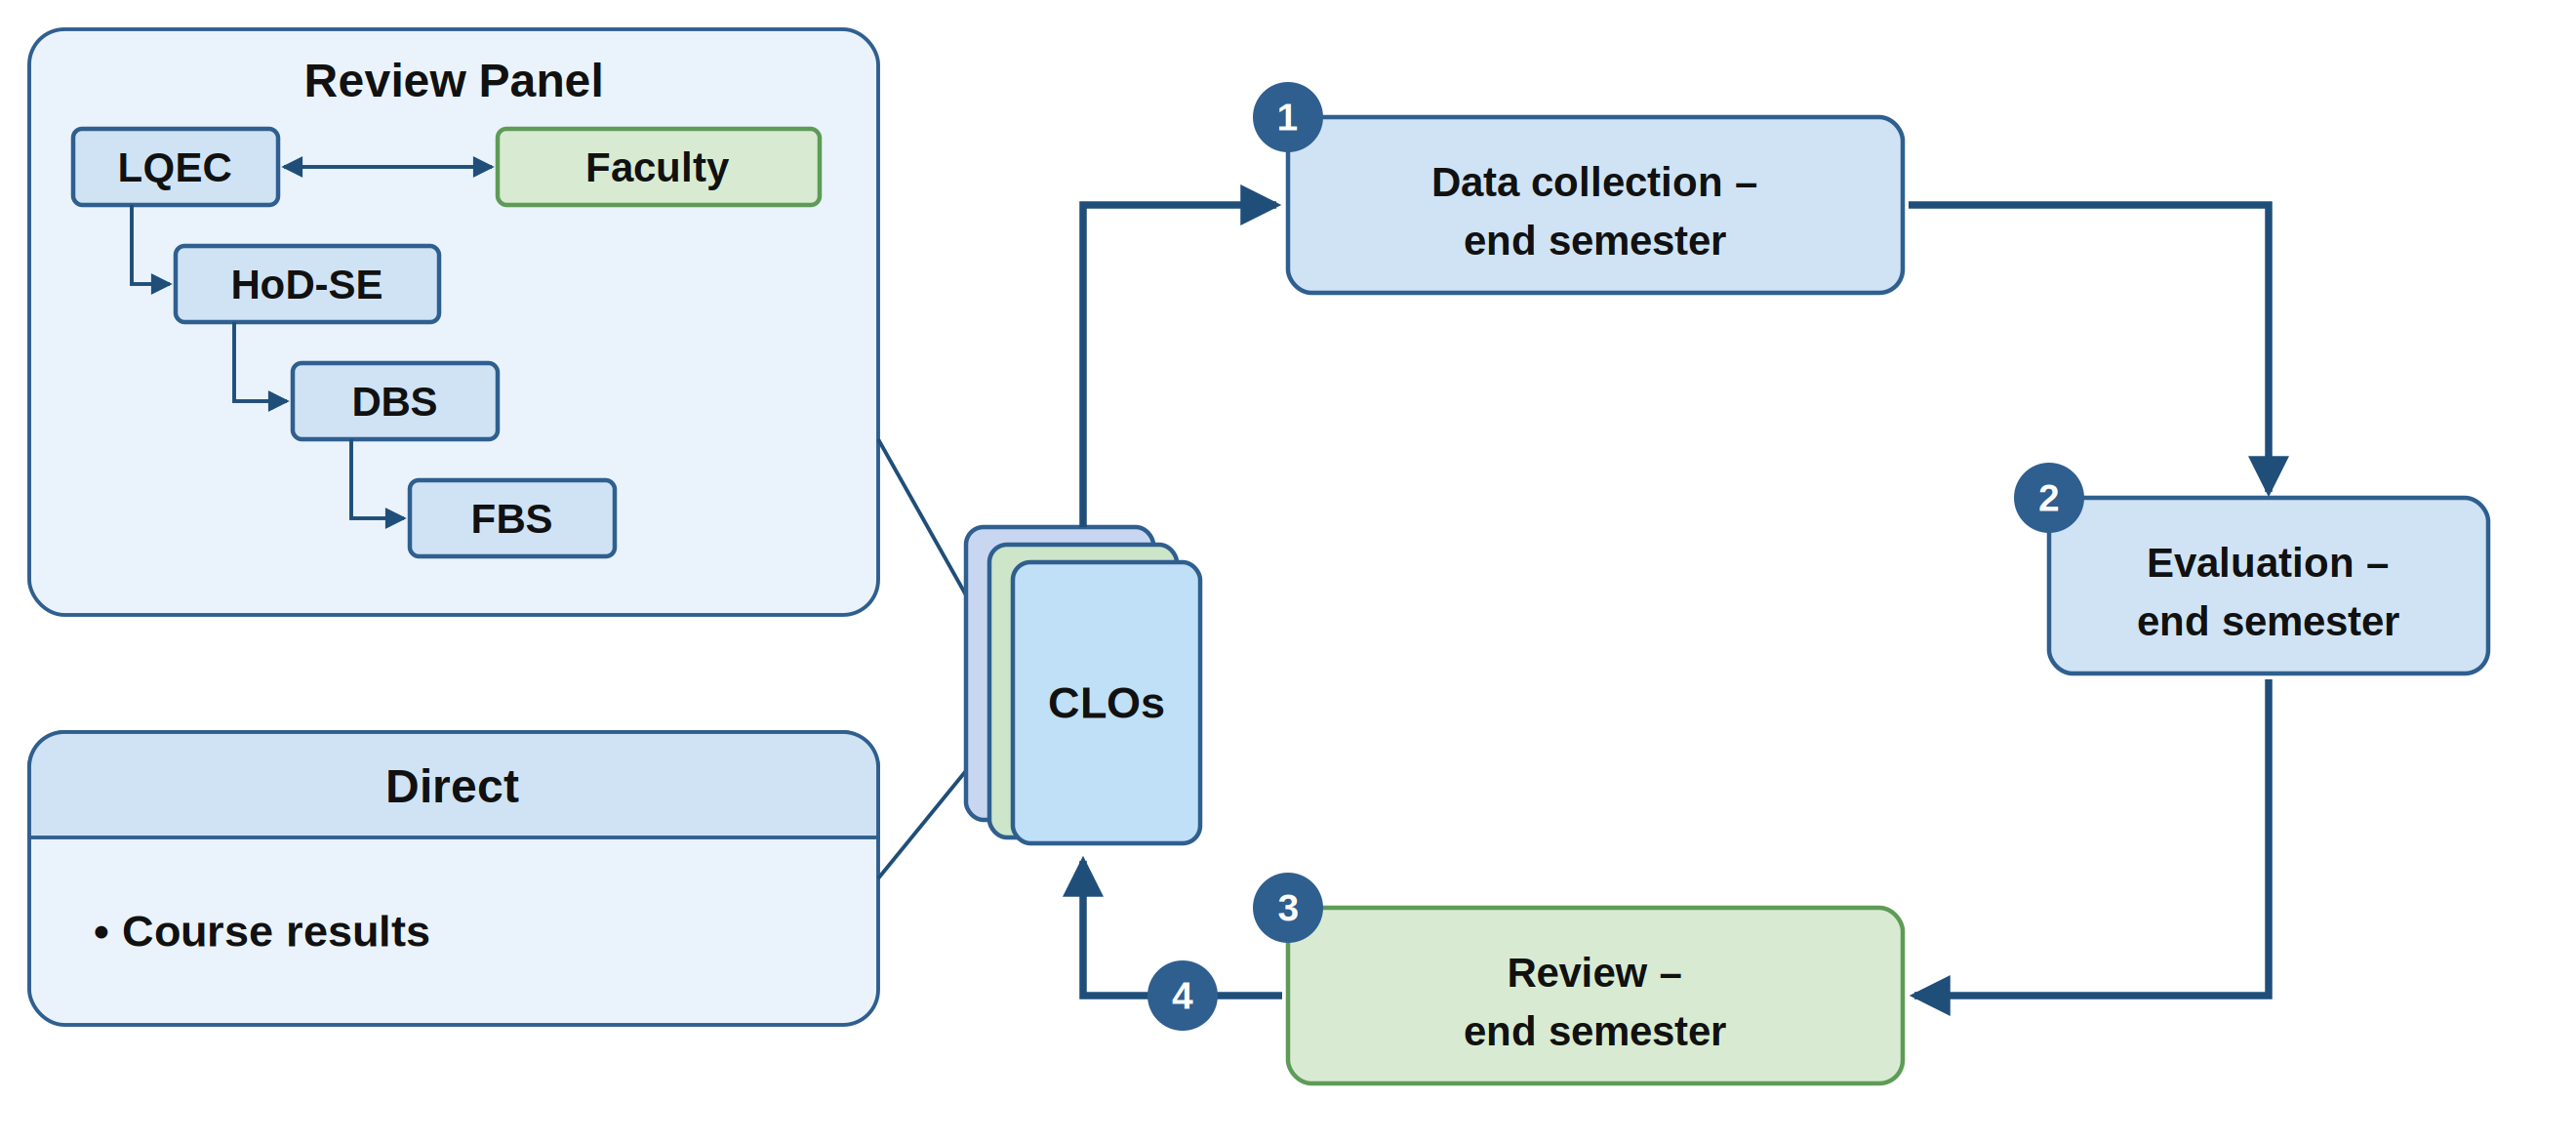
\includegraphics[width=1.0\textwidth]{images/front_matter/media/image-18.png}
\caption{Attainment and Review Process of CLOs}
\label{fig:cqi clo}
\end{figure}

CLOs are directly assessed through coursework and laboratory work involving examination and rubrics. For each course, the review process for attainment of CLOs is shown in Figure~\ref{fig:corrective CLOs}. If the cohort attainment of CLOs is equal to or more than 60\%, no corrective action is required. If cohort CLO attainment is less than 60\%, the corrective actions are invoked by the LQEC in consultation with the relevant faculty.
%\subsubsection{Review and Corrective Action Processes for CLOs}\label{review-and-corrective-action-processes-for-clos}

\begin{figure}[H]
\centering
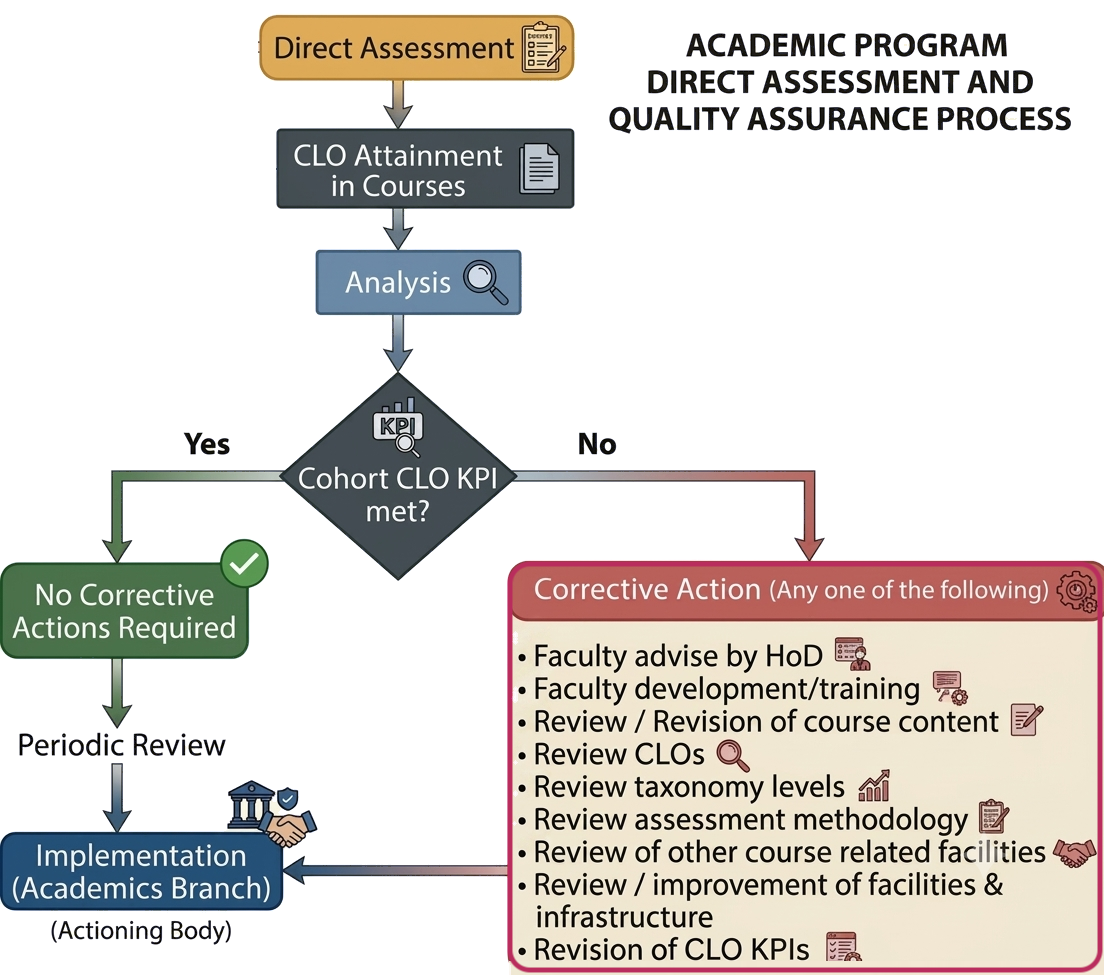
\includegraphics[width=5.18in,height=4.89in]{images/front_matter/media/image-19.png}
\caption{Corrective Actions for CLOs}
\label{fig:corrective CLOs}
\end{figure}

\section{Progress Since Last Accreditation Visit}\label{progress-on-last-accreditation-visit}

The previous PEC accreditation visit identified improvement opportunities across PEO assessment, PEO--PLO alignment, CLO/PLO mapping and taxonomy, indirect and direct assessment, and implementation of corrective actions. These observations have been addressed through the program's CQI mechanism. The complete institutional response to the previous visit is retained as Rejoinder under Criteria 8. The implementation status is discussed in Chapter~\ref{criterion-8-continual-quality-improvement} under Section~\ref{Implementation-Status-of-Previous-Accreditation-Observations}. To avoid duplicating the full rejoinder, Table~\ref{tab:last-visit-summary} summarizes the main action areas and points to the same supporting annexures used in Chapter~\ref{criterion-8-continual-quality-improvement}.

\begingroup
\footnotesize
\setlength{\tabcolsep}{4pt}
\renewcommand{\arraystretch}{1.15}
\begin{longtable}{@{}>{\raggedright\arraybackslash}p{0.24\textwidth}>{\raggedright\arraybackslash}p{0.48\textwidth}>{\raggedright\arraybackslash}p{0.20\textwidth}@{}}
\caption{Summary of Major Actions Following the Previous PEC Accreditation Visit}
\label{tab:last-visit-summary}\\
\toprule
\textbf{Area} & \textbf{Implemented Response} & \textbf{Supporting Evidence}\\
\midrule
\endfirsthead
\toprule
\textbf{Area} & \textbf{Implemented Response} & \textbf{Supporting Evidence}\\
\midrule
\endhead
\bottomrule
\endlastfoot
PEO assessment & Alumni and employer survey instruments were revised to improve question-to-PEO traceability and balanced coverage of the PEOs. & Chapter~\ref{criterion-1-program-educational-objectives}; Annexure A \\ %Annexure~\ref{revised-alumni-survey}; Annexure~\ref{revised-employ-survey}\\

\addlinespace[2pt]
PEO--PLO alignment & The PEO--PLO mapping was reviewed and updated, including explicit representation of innovation-related outcomes. & Chapter~\ref{criterion2}; Annexure B\\
%Chapter~\ref{sec:plopeo};Annexure~\ref{app:criteria-2_plo-peo_mapping_rationale}\\
\addlinespace[2pt]
CLO/PLO mapping and taxonomy & CLO wording, learning domains, Bloom's Taxonomy levels, and CLO--PLO mappings were reviewed through course and departmental CQI processes. &  Chapter~\ref{criterion2}\\
%Chapter~\ref{sec:cloplo}\\
\addlinespace[2pt]
Assessment and internship feedback & Direct-assessment practices and indirect assessment instruments, including internship feedback, were revised to strengthen outcome traceability and consistency. & Chapter~\ref{criterion2}; Chapter~\ref{criterion3}; Annexure B\\
%Chapter~\ref{sec:directassess}; Chapter~\ref{sec:indirectassess}; Chapter~\ref{sec:4.8internship}; Annexure~\ref{annex:internship-feedback-form}; Annexure~\ref{annex:graduate-exit-survey-form}\\
\addlinespace[2pt]
Corrective-action tracking & Corrective actions are documented and monitored through the formal CQI mechanism using Corrective Action Forms and follow-up review. & Chapter~\ref{criterion-8-continual-quality-improvement}\\
\addlinespace[2pt]
Curriculum response & Curriculum revisions arising from regulatory, assessment, and stakeholder inputs are processed through the approved academic governance mechanism. & Chapter~\ref{criterion3}\\
\end{longtable}
\endgroup

